\chapter{Байесовская дистилляция моделей глубокого обучения}
Исследуется проблема понижения сложности аппроксимирующих моделей. 
Рассматриваются методы, основанные на дистилляции моделей глубокого обучения. 
Вводятся понятия учителя и ученика. Предполагается, что модель ученика имеет меньшее число параметров, чем модель учителя. 
Предлагается байесовский подход к выбору модели ученика. 
Предложен метод назначения априорного распределения параметров ученика на основе апостериорного распределения параметров модели учителя. 
Так как пространства параметров учителя и ученика не совпадают, предлагается механизм выравнивания пространства параметров модели учителя и пространства параметров модели ученика путем изменения структуры модели учителя.
В данном разделе приводится теоретический анализ предложенного механизма выравнивания.

В данной главе представлены методы основанный на байесовском выводе.
В качестве априорного распределения параметров модели ученика предлагается использовать апостериорное распределение параметров модели учителя.
Решается задача выравнивание пространства параметров модели учителя и модели ученика.
Предлагается подход, основанный на последовательном выравнивании пространств параметров модели ученика и учителя. 
\begin{definition}
\label{def:structure}
Структура модели --- упорядоченный набор структурных параметров модели, которые задают вид суперпозиции.
\end{definition}
\begin{definition}
\label{def:sopos}
Выравнивание параметрических моделей --- изменение структуры модели (одной или нескольких моделей) в результате которого векторы параметров различных моделей лежат в одном пространстве.
\end{definition}
В следствие этого выравнивания в качестве априорного распределения параметров модели ученика выбирается апостериорное распределение параметров модели учителя.
В данной работе в качестве параметрической моделей рассматривается полносвязная нейронная сеть и рекурентная нейронная сеть.
В качестве структурных параметров модели выбраны число слоев, а также размер каждого скрытого слоя.

В рамках предложенного метода выравнивания параметрических моделей не оговорен выбор порядка на множестве параметров модели учителя.
Для этого предлагается упорядочивать параметры модели учителя на основе их релевантности.
Первый нейрон является наиболее релевантным, а последний нейрон наименее релевантным.
Порядок задается на основе отношения плотности распределения упорядочивваемого параметра к плотности распределения параметра в нуле~\cite{graves2011} или на основе метода Белсли~\cite{grabovoy2019}.

В рамках вычислительного эксперимента проводится теоретический анализ. Предложенный метод дистилляции анализируется на примере синтетической выборки, а также на реальной выборке FashionMnist~\cite{fashionmnist}.

\section{Постановка задачи дистилляции в терминах байесовского подхода}
Задана выборка
\[
\label{ch:3:eq:st:1}
\begin{aligned}
\mathfrak{D} = \left\{\left(\mathbf{x}_i, y_i\right)\right\}_{i=1}^{m}, \qquad \mathbf{x}_i \in \mathbb{R}^{n}, \quad y_i \in \mathbb{Y},
\end{aligned}
\]
где $\mathbf{x}_i, y_i$ --- признаковое описание и целевая переменная $i$-го объекта, число объектов в обучающей выборке обозначается $m$. Размер признакового описания объектов обозначается $n$. Множество $\mathbb{Y}=\{1,\ldots,R\}$ для задачи классификации, где $R$ число классов, множество $\mathbb{Y}=\mathbb{R}$ для задачи регрессии.

Задана модель учителя в виде суперпозиций линейных и нелинейных преобразований:
\[
\label{ch:3:eq:st:2}
\begin{aligned}
f = \bm{\sigma} \circ \mathbf{U}_T \bm{\sigma} \circ \mathbf{U}_{T-1}\circ \ldots  \mathbf{U}_2\bm{\sigma} \circ \mathbf{U}_1,
\end{aligned}
\]
где $T$ --- число слоев модели учителя, $\bm{\sigma}$ --- функция активации, а $\mathbf{U}_t$ обозначает матрицу линейного преобразования. Матрицы $\mathbf{U}$ соединяются в вектор параметров $\mathbf{u}$ модели учителя $f$:
\[
\label{ch:3:eq:st:2.1}
\begin{aligned}
\mathbf{u} = \text{vec}\bigr(\left[\mathbf{U}_T, \mathbf{U}_{T-1}, \ldots \mathbf{U}_1\right]\bigr),
\end{aligned}
\]
где $\text{vec}$ операция векторизации соединенных матриц.
Каждая матрица $\mathbf{U}_t$ имеет размер $n_t\times n_{t-1},$ где $n_0=n,$ а  $n_T={1}$ для задачи регрессии и $n_T=R$ для задачи классификации на $R$ классов. Число параметров $N_{\text{tr}}$ учителя $f$
\[
\label{ch:3:eq:st:2.2}
\begin{aligned}
N_{\text{tr}} = \sum_{t=1}^{T}n_tn_{t-1}.
\end{aligned}
\]
Для построения вектора параметров $\mathbf{u}$ задается полный порядок на элементов матриц $\mathbf{U}_t$. Для полносвязнной нейронной сети вводится естественный порядок, индуцированный номером слоя $t$, номером нейрона, и номером элемента вектора параметров нейрона: выбирается матрица $\mathbf{U}_t$, строка этой матрицы и элемент строки.

Например, для модели учителя в задаче регрессии:
\[
\label{ch:3:eq:st:3}
\begin{aligned}
f\bigr(\mathbf{x}\bigr) = \bm{\sigma} \circ \mathbf{U}_3 \bm{\sigma} \circ \mathbf{U}_2\bm{\sigma}\circ \mathbf{U}_1\mathbf{x},
\end{aligned}
\]
вектор параметров $\mathbf{u}$ принимает вид
\[
\label{ch:3:eq:st:4}
\begin{aligned}
\mathbf{u} = \bigr[u_1^{1,1}, \ldots, u_1^{1,n},
                                               \ldots, 
                             u_1^{n_1,1}, &\ldots, u_1^{n_1,n},  
                             u_2^{1, 1}, \ldots, u_2^{1, n_1}, \\
                                                & \ldots, 
                            u_2^{n_2, 1}, \ldots, u_2^{n_2, n_1},
                            u_3^{1, 1}, \ldots, u_3^{1, n_2}\bigr].
\end{aligned}
\]
Пусть для вектора параметров учителя $f$ известно апостериорное распределение параметров $p\bigr(\mathbf{u}|\mathfrak{D}\bigr)$. 
На основе выборки $\mathfrak{D}$ и апостериорного распределения параметров учителя $f$ требуется выбрать модель ученика из параметрического семейства функций:
\[
\label{ch:3:eq:st:5}
\begin{aligned}
g = \bm{\sigma} \circ \mathbf{W}_L\bm{\sigma}  \circ \ldots \circ \mathbf{W}_1, \quad \mathbf{W}_l \in \mathbb{R}^{n_l \times n_{l-1}},
\end{aligned}
\]
где $L$ число слоев модели ученика.
Число параметров $N_{\text{st}}$ модели ученика $g$ вычисляется аналогично выражению \eqref{ch:3:eq:st:2.2}.
Вектор параметров модели ученика $\mathbf{w}$ строится аналогичным образом \eqref{ch:3:eq:st:2.1}.
Модель $g$ задается своим вектором параметров $\mathbf{w}$.
Следовательно, задача выбора модели $g$ эквивалентна задаче оптимизации вектора параметров $\mathbf{w}\in\mathbb{R}^{N_{\text{st}}}$.

Параметры $\hat{\mathbf{w}} \in \mathbb{R}^{N_{\text{st}}}$ оптимизируются при помощи вариационного вывода на основе совместного правдоподобия модели и данных:
\[
\label{ch:3:eq:st:6}
\begin{aligned}
\mathcal{L}\bigr(\mathfrak{D}, \mathbf{A}\bigr) = \log p\bigr(\mathfrak{D}|\mathbf{A}\bigr) = \log \int_{\mathbf{w} \in \mathbb{R}^{N_{\text{st}}}}p\bigr(\mathfrak{D}|\mathbf{w}\bigr)p\bigr(\mathbf{w}|\mathbf{A}\bigr)d\mathbf{w},
\end{aligned}
\]
где $p\bigr(\mathbf{w}| \mathbf{A}\bigr)$ --- априорное распределение вектора параметров модели ученика.
Так как взятие интеграла \eqref{ch:3:eq:st:6} является вычислительно сложной задачей, используется вариационный вывод~\cite{graves2011, grabovoy2019}. Для этого задается вариационное распределение параметров модели ученика $q\bigr(\mathbf{w}|\bm{\mu}, \bm{\Sigma}\bigr),$ которое аппроксимирует неизвестное апостериорное распределение $p\bigr(\mathbf{w}|\mathfrak{D}\bigr)$
\[
\label{ch:3:eq:st:new:1}
\begin{aligned}
q\bigr(\mathbf{w}|\bm{\mu}, \bm{\Sigma}\bigr) \approx  p\bigr(\mathbf{w}|\mathfrak{D}\bigr).
\end{aligned}
\]
Оптимизация параметров $\mathbf{w}$ сводится к решению  задачи:
\[
\label{ch:3:eq:st:7}
\begin{aligned}
\hat{\mathbf{w}} = \arg \min_{\bm{\mu}, \bm{\Sigma}, \mathbf{w}} \text{D}_{\text{KL}}\bigr(q\bigr(\mathbf{w}|\bm{\mu}, \bm{\Sigma}\bigr)||p\bigr(\mathbf{w}|\mathbf{A}\bigr)\bigr) - \log p\bigr(\mathbf{y}|\mathbf{X}, \mathbf{w}\bigr).
\end{aligned}
\]
Выражение~\eqref{ch:3:eq:st:7} не учитывает параметры учителя $f\bigr(\mathbf{x}, \mathbf{u}\bigr)$. Для использования параметров учителя при решении оптимизационной задачи\eqref{ch:3:eq:st:7} предлагается рассмотреть зависимость параметров априорного распределения $p\bigr(\mathbf{w}|\mathbf{A}\bigr)$ от параметров апостериорного распределения учителя $p\bigr(\mathbf{u}|\mathfrak{D}\bigr)$.

\section{Выравнивание априорного распределения параметров ученика на основе параметров учителя}
Апостериорное распределение параметров модели учителя предполагается нормальным:
\[
\label{ch:3:eq:ap:1}
\begin{aligned}
p\bigr(\mathbf{u}|\mathfrak{D}\bigr) = \mathcal{N}\bigr(\mathbf{m}, \bm{\Sigma}\bigr),
\end{aligned}
\]
где $\mathbf{m}$ и $\bm{\Sigma}$ параметры этого распределения. На основе параметров $\mathbf{m}$ и $\bm{\Sigma}$ требуется задать параметры $\mathbf{A}$ априорного распределения $p\bigr(\mathbf{w}|\mathbf{A}\bigr).$
Структуры моделей учителя и ученика задаются числом слоев и размером этих слоев, то возможны варианты: 1) число слоев и размер каждого слоя совпадает; 2) число слоев совпадает, а размеры различаются; 3) не совпадает число слоев.

\paragraph{Учитель и ученик принадлежат одному семейству.}
\label{section:one:space}
Рассмотрим условия:
\begin{enumerate}[1)]
    \item число слоев модели учителя равняется числу слоев модели ученика $L=T$;
    \item размеры соответствующих слоев совпадают, другими словами, для всех $t, l$ таких, что $t=l$ выполняется $n_l = n_t,$ где $n_t$ обозначает размер $t$-го слоя учителя, а $n_l$ размер $l$-го слоя ученика.
\end{enumerate}
При выполнении этих условий, априорное распределение параметров модели ученика приравнивается к апостериорному распределения параметров учителя $p\bigr(\mathbf{w}|\mathbf{A}\bigr) = p\bigr(\mathbf{u}|\mathfrak{D}\bigr)$.

\paragraph{Удаление нейрона в слое учителя.}
Проведем выравнивание модели учителя и модели ученика, согласно определению \ref{def:sopos} при помощи последовательных преобразований параметров $\mathbf{u}$. Рассмотрим преобразование
\[
\label{ch:3:eq:ap:2}
\begin{aligned}
\bm{\phi}\bigr(t, \mathbf{u}\bigr) : \mathbb{R}^{N_{\text{tr}}} \to \mathbb{R}^{N_{\text{tr}}-2n_t}
\end{aligned}
\]
вектора $\mathbf{u},$ которое описывает удаление одного нейрона из $t$-го слоя учителя.
Обозначим новый вектор параметров $\bm{\upsilon} =  \bm{\phi}\bigr(t, \mathbf{u}\bigr),$ а элементы вектора, которые удалены как $\bar{\bm{\upsilon}}.$ Заметим, что векторы $\bm{\upsilon}$ и $\bar{\bm{\upsilon}}$ являются случайными величинами. 

\begin{theorem}
Пусть задано распределение вектора параметров~$p\bigr(\mathbf{u}\bigr).$ Тогда распределение вектора параметров~$p\bigr(\bm{\upsilon}\bigr)$ представимо в виде:
\[
p\bigr(\bm{\upsilon}\bigr)  = \int\limits_{ \bm{\nu}_2 \in \mathbb{R}^{n_{t-1}}}p\bigr(\bar{\bm{\nu}}_1|\mathfrak{D}, \bm{\nu}_1=\mathbf{0}\bigr) d \bm{\nu}_2.
\]
\end{theorem}
\begin{proof}
Пусть $\bm{\phi}\bigr(t, \mathbf{u}\bigr)$ удаляет $j$-й нейрон в $t$-м слое, что является удалением $j$-й строки матрицы $\mathbf{U}_t$. Заметим, что удаление $j$-й строки матрицы $\mathbf{U}_t$ влечет удаление $j$-й компоненты вектора $z_{t+1}$, где
\[
\label{ch:3:eq:ap:tr:neural:1}
\begin{aligned}
\mathbf{z}_{t} = \bm{\sigma} \circ \mathbf{U}_{t-1} \bm{\sigma} \circ \ldots  \mathbf{U}_2\bm{\sigma} \circ \mathbf{U}_1\mathbf{x}.
\end{aligned}
\]

Удаление $j$-й компоненты вектора $\mathbf{z}_{t+1}$ эквивалентно занулению $j$-го столбца матрицы $\mathbf{U}_{t+1}.$ Заметим, что тогда предсказание модели не зависит от параметров $j$-й строки матрицы $\mathbf{U}_t,$ а следовательно данными параметрами также можно пренебречь.

Найдем распределение вектора $\bm{\upsilon}.$ Для поиска распределения вектора параметров после зануления $j$-го столбца матрицы $\mathbf{U}_{t+1}$ воспользуемся формулой условной вероятности $p\bigr(\bar{\bm{\nu}}_1|\mathfrak{D}, \bm{\nu}_1=\mathbf{0}\bigr)$, а для удаления $j$-й строки матрицы $\mathbf{U}_{t}$ воспользуемся маргинализацией распределения $p\bigr(\bar{\bm{\nu}}_1|\mathfrak{D}, \bm{\nu}_1=\mathbf{0}\bigr)$. Обозначим зануляемые параметры модели как $\bm{\nu}_1,$ а удаляемые параметры как $\bm{\nu}_2.$ Также обозначим все параметры, которые не занулены как $\bar{\bm{\nu}}_1 = [\bm{\upsilon}^{\mathsf{T}}, \bm{\nu}_2^{\mathsf{T}}].$ Итоговое распределение параметров принимает  вид:
\[
\label{ch:3:eq:ap:tr:1:1}
\begin{aligned}
p\bigr(\bm{\upsilon}|\mathfrak{D}\bigr)  = \int_{\bm{\nu}_2}p\bigr(\bar{\bm{\nu}}_1|\mathfrak{D}, \bm{\nu}_1=\mathbf{0}\bigr) d\bm{\nu}_2.
\end{aligned}
\]
\end{proof}

\begin{theorem}
\label{theorem:ap:neural}
Пусть выполняются условия:
\begin{enumerate}[1)]
\item апостериорное распределение параметров $p\bigr(\mathbf{u}|\mathfrak{D}\bigr) = \mathcal{N}\bigr(\mathbf{m}, \bm{\Sigma}\bigr),$
\item число слоев модели учителя равняется числу слоев модели ученика $T=L$,
\item размеры соответствующих слоев не совпадают, другими словами, для всех $t, l,$ таких что $t=l,$ выполняется $n_t \geq n_l.$
\end{enumerate}
Тогда распределение параметров~$p\bigr(\bm{\upsilon}|\mathfrak{D}\bigr)$ также является нормальным.
\end{theorem}
\begin{proof}
Из свойств нормального распределения следует, что распределение
\[
\label{ch:3:eq:ap:tr:neural:2}
\begin{aligned}
p\bigr(\bar{\bm{\nu}}_1|\mathfrak{D}, \bm{\nu}_1=\mathbf{0}\bigr)
\end{aligned}
\]
также является нормальным распределением с параметрами $\bm{\mu}, \bm{\Xi}$:
\[
\label{ch:3:eq:ap:tr:1:1}
\begin{aligned}
\bm{\mu} &= \mathbf{m}_{\bar{\bm{\nu}}_1}+\bm{\Sigma}_{\bar{\bm{\nu}}_1,\bm{\nu}_1} \bm{\Sigma}_{\bm{\nu}_1,\bm{\nu}_1}^{-1} \left(\mathbf{0} - \mathbf{m}_{\bm{\nu}_1}\right), \\
 \bm{\Xi} &= \bm{\Sigma}_{\bar{\bm{\nu}}_1,\bar{\bm{\nu}}_1} - \bm{\Sigma}_{\bar{\bm{\nu}}_1,\bm{\nu}_1} \bm{\Sigma}_{\bm{\nu}_1,\bm{\nu}_1}^{-1} \bm{\Sigma}_{\bar{\bm{\nu}}_1,\bm{\nu}_1},
\end{aligned}
\]
где векторы $\mathbf{m}_{\bar{\bm{\nu}}_1}, \mathbf{m}_{\bm{\nu}_1}$ являются подвекторами вектора $\mathbf{m},$ который относится к параметрам $\bar{\bm{\nu}}_1$ и $\bm{\nu}_1$ соответсвенно. Ковариационная матрица $\bm{\Sigma}_{\bar{\bm{\nu}}_1,\bm{\nu}_1}$ обозначает подматрицу матрицы $\bm{\Sigma},$ которая соответсвует ковариационной матрицей между параметрами $\bar{\bm{\nu}}_1$ и $\bm{\nu}_1.$

Распределение $p\bigr(\bm{\upsilon}|\mathfrak{D}\bigr)$ найдем при помощи маргинализации распределения \eqref{ch:3:eq:ap:tr:neural:2} по параметрам $\bm{\nu}_2.$ Используя свойства нормального распределения получаем распределения:
\[
\label{ch:3:eq:ap:3}
\begin{aligned}
p\bigr(\bm{\upsilon}|\mathfrak{D}\bigr) = \mathcal{N}\bigr(\bm{\mu}_{\bm{\upsilon}},  \bm{\Xi}_{\bm{\upsilon}, \bm{\upsilon}}\bigr),
\end{aligned}
\]
где $\bm{\mu}_{\bm{\upsilon}}$ обозначает подвектор вектора $\bm{\mu},$ который относится к параметру $\bm{\upsilon}$, а матрица $\bm{\Xi}_{\bm{\upsilon}, \bm{\upsilon}}$ является подматрицей матрицы $\bm{\Xi}$, которая относится к вектору параметрамов $\bm{\upsilon}.$
\end{proof}

Теорема \ref{theorem:ap:neural} задает апостериорное распределение параметров \eqref{ch:3:eq:ap:3} после зануления нейронов в модели нейросети --- учителя. Заметим, что аналогичным образом можно удалить подмножество нейронов в одном слое. Если число нейронов отличается в нескольких слоях модели нейросети учителя, то выполняется последовательно применения отображения $\bm{\phi}\bigr(t, \mathbf{u}\bigr)$ для каждого $t$-го слоя.


Приведем пояснение доказательства теоремы. Введем обозначение:

\[
\hat{\mathbf{w}}, \hat{\bm{\mu}}, \hat{\bm{\Sigma}} = \arg \min_{\bm{\mu}, \bm{\Sigma}, \mathbf{w}} \text{D}_{\text{KL}}\bigr(q\bigr(\mathbf{w}|\bm{\mu}, \bm{\Sigma}\bigr)||p\bigr(\mathbf{w}|\mathbf{A}\bigr)\bigr) - \sum_{i=1}^{m}\log p\bigr(y_i|\mathbf{x}_{i}, \mathbf{w}\bigr).
\]
Параметры~$\mathbf{u}$ модели~$\mathbf{f}$ делятся на {\color{red} удаляемые~$\bm{\nu}_2$}, {\color{blue} зануляемые~$\bm{\nu}_1$}, {оставшиеся~$\bm{\upsilon}$}.

Суперпозиция слоев модели учителя~$\mathbf{f}$ в окрестности~$t$-го слоя:
{\small
\[
\mathbf{f}\bigr(\mathbf{x}\bigr) = \ldots \circ
\underbrace{
\begin{pmatrix}
u_{1,1} & \ldots & {\color{blue} u_{1,j}} & \ldots & u_{1,n_{t}} \\
\vdots  & \ddots & {\color{blue} \vdots}  & \ddots & \vdots \\
u_{n_{t+1},1} & \ldots & {\color{blue} u_{n_{t+1},j}} & \ldots & u_{n_{t+1},n_{t}} \\
\end{pmatrix} 
}_{\mathbf{U}_{t+1}}
\bm{\sigma} 
\circ 
\underbrace{
\begin{pmatrix}
u_{1,1} & \ldots & u_{1,n_{t-1}} \\
\vdots  & \ddots & \vdots        \\
{\color{red} u_{j,1}} & {\color{red}\ldots} & {\color{red} u_{j,n_{t-1}}} \\
\vdots  & \ddots & \vdots        \\
u_{n_{t},1} & \ldots & u_{n_{t},n_{t-1}} \\
\end{pmatrix}
}_{\mathbf{U}_{t}}
\bm{\sigma}
\circ 
\ldots
\circ 
\mathbf{U}_1
\mathbf{x}
\]
}
Апостериорное распределение параметров~$\bm{\upsilon}$ модели~$\mathbf{f}$:
\[
p\bigr(\bm{\upsilon}|\mathfrak{D}\bigr)  = \int\limits_{{\color{red} \bm{\nu}_2} \in \mathbb{R}^{n_{t-1}}}p\bigr({\color{blue}\bar{\bm{\nu}}_1}|\mathfrak{D}, {\color{blue}\bm{\nu}_1}=\mathbf{0}\bigr) d{\color{red} \bm{\nu}_2}.
\]
Из свойства распределения 
\[
    p\bigr(\bar{\bm{\nu}}_1|\mathfrak{D}, \bm{\nu}_1=\mathbf{0}\bigr) = \mathcal{N}\bigr(\bm{\mu}, \bm{\Xi}\bigr),
\]
с параметрами~$\bm{\mu}, \bm{\Xi}$:
\[
\begin{aligned}
\bm{\mu} &= \mathbf{m}_{\bar{\bm{\nu}}_1}+\bm{\Sigma}_{\bar{\bm{\nu}}_1,\bm{\nu}_1} \bm{\Sigma}_{\bm{\nu}_1,\bm{\nu}_1}^{-1} \left(\mathbf{0} - \mathbf{m}_{\bm{\nu}_1}\right), \\
 \bm{\Xi} &= \bm{\Sigma}_{\bar{\bm{\nu}}_1,\bar{\bm{\nu}}_1} - \bm{\Sigma}_{\bar{\bm{\nu}}_1,\bm{\nu}_1} \bm{\Sigma}_{\bm{\nu}_1,\bm{\nu}_1}^{-1} \bm{\Sigma}_{\bar{\bm{\nu}}_1,\bm{\nu}_1}.
\end{aligned}
\]
Маргинализация нормального распределения
\[
p\bigr(\bm{\upsilon}|\mathfrak{D}\bigr) = \mathcal{N}\bigr(\bm{\mu}_{\bm{\upsilon}},  \bm{\Xi}_{\bm{\upsilon}, \bm{\upsilon}}\bigr),
\]
что соответствует полученному в теореме~\ref{theorem:ap:neural}.

\paragraph{Удаление слоя учителя.}
Проведем выравнивание модели учителя и модели ученика, согласно определению \ref{def:sopos} при помощи последовательных преобразований вектора параметров $\mathbf{u}$. Рассмотрим преобразование:
\[
\label{ch:3:eq:ap:4}
\begin{aligned}
\bm{\psi}\bigr(t, \mathbf{u}\bigr) : \mathbb{R}^{N_{\text{tr}}} \to \mathbb{R}^{N_{\text{tr}}-n_tn_{t-1}}
\end{aligned}
\]
вектора $\mathbf{u}$ которое описывает удаление одного $t$-го слоя.
Обозначим новый вектор параметров $\bm{\upsilon} = \bm{\psi}\bigr(t, \mathbf{u}\bigr),$ а элементы вектора, которые удалены как $\bar{\bm{\upsilon}}.$ 

\begin{theorem}
\label{theorem:ap:layer}
Пусть выполняются условия:
\begin{enumerate}[1)]
\item апостериорное распределение параметров $p\bigr(\mathbf{u}|\mathfrak{D}\bigr) = \mathcal{N}\bigr(\mathbf{m}, \bm{\Sigma}\bigr),$
\item соответствующие размеры слоев совпадают, $n_t=n_{t-1},$ т.е. матрица~$\mathbf{U}_t$ является квадратной,
\item функция активации удовлетворяет свойству идемпотентности $\bm{\sigma} \circ \bm{\sigma} = \bm{\sigma}$.
\end{enumerate}
Тогда апостериорное распределение также описывается нормальным распределением с плотностью распределения
\[
\label{ch:3:eq:ap:5}
\begin{aligned}
p\bigr(\bm{\upsilon}|\mathfrak{D}\bigr) = \mathcal{N}\bigr(\mathbf{m}_{\bm{\upsilon}}+\bm{\Sigma}_{\bm{\upsilon},\bar{\bm{\upsilon}}} \bm{\Sigma}_{\bar{\bm{\upsilon}},\bar{\bm{\upsilon}}}^{-1} \left(\mathbf{i} - \bar{\bm{\upsilon}}\right), \bm{\Sigma}_{\bm{\upsilon},\bm{\upsilon}} - \bm{\Sigma}_{\bm{\upsilon},\bar{\bm{\upsilon}}}\bm{\Sigma}_{\bar{\bm{\upsilon}},\bar{\bm{\upsilon}}}^{-1}\bm{\Sigma}_{\bm{\upsilon},\bar{\bm{\upsilon}}}\bigr),
\end{aligned}
\]
где
\[
\mathbf{i}=[\underbrace{1, 0, \ldots, 0}_{n_t}, \underbrace{0, 1, \ldots, 0}_{n_t}, \underbrace{0, 0, 1, \ldots, 0}_{n_t}, \underbrace{0, \ldots, 1}_{n_t}]^{\mathsf{T}}.
\]
\end{theorem}
\begin{proof}
Рассмотрим две структуры нейронной сети с $T$ слоями и $T+1$ слоем соответственно. Рассмотрим $t$-й слой, для которого выполняются условия этой теоремы. Заметим, что если $t$-й слой нейронной сети с $T+1$ слоем приравнять к единичной матрице, то он будет эквивалентным архитектуре с $T$ слоями:
\[
\begin{aligned}
f &= \bm{\sigma} \circ \mathbf{U}_{T+1}\bm{\sigma} \circ \mathbf{U}_T \ldots \bm{\sigma} \circ \mathbf{U}_t\bm{\sigma} \circ \ldots  \mathbf{U}_2\bm{\sigma} \circ \mathbf{U}_1 =\\
&=  \bm{\sigma} \circ \mathbf{U}_{T+1}\bm{\sigma} \circ \mathbf{U}_T \ldots \bm{\sigma} \circ \mathbf{I}\bm{\sigma} \circ \ldots  \mathbf{U}_2\bm{\sigma} \circ \mathbf{U}_1 =\\
&=  \bm{\sigma} \circ \mathbf{U}_{T+1}\bm{\sigma} \circ \mathbf{U}_T \ldots \bm{\sigma} \circ \bm{\sigma} \circ \ldots  \mathbf{U}_2\bm{\sigma} \circ \mathbf{U}_1.
\end{aligned}
\]
Используя свойство идемпотентности функции~$\bm{\sigma}$ получаем:
\[
\label{ch:3:eq:ap:tr:2:1}
\begin{aligned}
f &= \bm{\sigma} \circ \mathbf{U}_{T+1}\bm{\sigma} \circ \mathbf{U}_T \ldots \bm{\sigma} \circ \ldots  \mathbf{U}_2\bm{\sigma} \circ \mathbf{U}_1.
\end{aligned}
\]
Получаем, что удаление $t$-го слоя нейросети эквивалентно приравниванию матрицы параметров $t$-го слоя к единичной матрице. Распределение параметров после приравнивая к единичной матрице вычисляется при помощи условного распределения. В силу общих свойств нормального распределения, условное распределения также является нормальным распределением с параметрами $\bm{\mu}, \bm{\Xi}:$
\[
\label{ch:3:eq:ap:tr:2:2}
\begin{aligned}
\bm{\mu} &= \mathbf{m}_{\bm{\upsilon}}+\bm{\Sigma}_{\bm{\upsilon},\bar{\bm{\upsilon}}} \bm{\Sigma}_{\bar{\bm{\upsilon}},\bar{\bm{\upsilon}}}^{-1} \left(\mathbf{i} - \bar{\bm{\upsilon}}\right), \\
\bm{\Xi} &= \bm{\Sigma}_{\bm{\upsilon},\bm{\upsilon}} - \bm{\Sigma}_{\bm{\upsilon},\bar{\bm{\upsilon}}}\bm{\Sigma}_{\bar{\bm{\upsilon}},\bar{\bm{\upsilon}}}^{-1}\bm{\Sigma}_{\bm{\upsilon},\bar{\bm{\upsilon}}}\bigr),
\end{aligned}
\]
где вектор $\mathbf{m}_{\bm{\upsilon}}$ является подвектором вектора $\mathbf{m}$ соответсвующий параметрам $\bm{\upsilon},$ а матрица $\bm{\Sigma}_{\bm{\upsilon},\bar{\bm{\upsilon}}}$ является подматрицей ковариационной матрицы $\bm{\Sigma}$ соответсвующий векторам параметров $\bm{\upsilon}$ и $\bar{\bm{\upsilon}}.$
\end{proof}

Теорема \ref{theorem:ap:layer} задает апостериорное распределение \eqref{ch:3:eq:ap:5} параметров после удаления слоя нейросети. Полученное распределение $p\bigr(\bm{\upsilon}|\mathfrak{D}\bigr) $ является оценкой апостериорного распределения модели без одного слоя.

\paragraph{Выравнивание рекурентных сетей.} Структура модели RNN задается размерностью скрытых слоев~$n_1, n_2, \ldots, n_T.$ Скрытое представление~$q$-го элемента последовательности~$h^{q}_{t}$ для~$t$-го слоя задается выражением:
\[
    \mathbf{h}^{q}_t = \sigma\bigr(\mathbf{U}^{1}_{t}\mathbf{h}^{q}_{t-1}+\mathbf{U}^{2}_{t}\mathbf{h}^{q-1}_{t}\bigr),
\]
где матрицы~$\left\{\mathbf{U}^{1}_{t}, \mathbf{U}^{2}_{t}\right\}_{t=1}^{T}$ задают матрицы линейных отображений в модели RNN.

Отображение
\[
\bm{\phi}_{\text{RNN}}\bigr(t, \mathbf{u}\bigr) : \mathbb{R}^{\text{p}_{\text{tr}}} \to \mathbb{R}^{\text{p}_{\text{tr}}-3n_t}
\]
описывает снижение размерности пространства после~$t$-го слоя на единицу. Полученный вектор параметров после снижения размерности обозначается:
\[
\bm{\upsilon} = \bm{\phi}\bigr(t, \mathbf{u}\bigr).
\]
Исходный вектор~$\mathbf{u}$ состоит из подвекторов $\bm{\nu}_2, {\bm{\nu}}_1, \bm{\upsilon},$ которые описывают удаляемые, зануляемые и оставшиеся параметры соответственно.

\begin{theorem}
Пусть задано распределение вектора параметров~$p\bigr(\mathbf{u}\bigr).$ Тогда распределение вектора параметров~$p\bigr(\bm{\upsilon}\bigr)$ представимо в виде:
\[
p\bigr(\bm{\upsilon}\bigr)  = \int\limits_{ \bm{\nu}_2 \in \mathbb{R}^{n_{t-1}}}p\bigr(\bar{\bm{\nu}}_1|\mathfrak{D}, \bm{\nu}_1=\mathbf{0}\bigr) d \bm{\nu}_2.
\]
\end{theorem}
\begin{proof}
Пусть~$\bm{\phi}\bigr(t, \mathbf{u}\bigr)$ удаляет~$j$-ю компоненту вектора скрытого представления~$\mathbf{h}^{q}_{t}.$ Удаление~$j$-й компоненты вектора~$\mathbf{h}^{q}_{t}$ эквивалентно занулению~$j$-го столбца матрицы~$\mathbf{U}^{1}_{t+1}.$ Тогда предсказания модели не заввисит от параметров в~$j$-й строке матрицы~$\mathbf{U}^{1}_{t}$ и~$\mathbf{U}^2_{t},$ а следовательно этими параметрами можно пренебречь.

Найдем распределение вектора $\bm{\upsilon}.$ Для поиска распределения вектора параметров после зануления $j$-го столбца матрицы $\mathbf{U}^{1}_{t+1}$ воспользуемся формулой условной вероятности $p\bigr(\bar{\bm{\nu}}_1|\mathfrak{D}, \bm{\nu}_1=\mathbf{0}\bigr)$, а для удаления $j$-й строки матриц $\mathbf{U}^{1}_{t}$ и $\mathbf{U}^{2}_{t}$ воспользуемся маргинализацией распределения $p\bigr(\bar{\bm{\nu}}_1|\mathfrak{D}, \bm{\nu}_1=\mathbf{0}\bigr)$. Обозначим зануляемые параметры модели как $\bm{\nu}_1,$ а удаляемые параметры как $\bm{\nu}_2.$ Также обозначим все параметры, которые не занулены как $\bar{\bm{\nu}}_1 = [\bm{\upsilon}^{\mathsf{T}}, \bm{\nu}_2^{\mathsf{T}}].$ Итоговое распределение параметров принимает  вид:
\[
\begin{aligned}
p\bigr(\bm{\upsilon}|\mathfrak{D}\bigr)  = \int_{\bm{\nu}_2}p\bigr(\bar{\bm{\nu}}_1|\mathfrak{D}, \bm{\nu}_1=\mathbf{0}\bigr) d\bm{\nu}_2.
\end{aligned}
\]
\end{proof}

\begin{theorem}
Пусть выполняются условия:
\begin{enumerate}
\item[1)] апостериорное распределение параметров $p\bigr(\mathbf{u}|\mathfrak{D}\bigr) = \mathcal{N}\bigr(\mathbf{m}, \bm{\Sigma}\bigr),$
\item[2)] число слоев модели учителя равняется числу слоев модели ученика $T=L$,
\item[3)] размеры соответствующих пространств не совпадают~$n_t \geq n_t.$
\end{enumerate}
Тогда распределение параметров~$p\bigr(\bm{\upsilon}|\mathfrak{D}\bigr)$ также является нормальным.
\end{theorem}
\begin{proof}
Из свойств нормального распределения следует, что распределение
\[
\begin{aligned}
p\bigr(\bar{\bm{\nu}}_1|\mathfrak{D}, \bm{\nu}_1=\mathbf{0}\bigr)
\end{aligned}
\]
также является нормальным распределением с параметрами $\bm{\mu}, \bm{\Xi}$:
\[
\begin{aligned}
\bm{\mu} &= \mathbf{m}_{\bar{\bm{\nu}}_1}+\bm{\Sigma}_{\bar{\bm{\nu}}_1,\bm{\nu}_1} \bm{\Sigma}_{\bm{\nu}_1,\bm{\nu}_1}^{-1} \left(\mathbf{0} - \mathbf{m}_{\bm{\nu}_1}\right), \\
 \bm{\Xi} &= \bm{\Sigma}_{\bar{\bm{\nu}}_1,\bar{\bm{\nu}}_1} - \bm{\Sigma}_{\bar{\bm{\nu}}_1,\bm{\nu}_1} \bm{\Sigma}_{\bm{\nu}_1,\bm{\nu}_1}^{-1} \bm{\Sigma}_{\bar{\bm{\nu}}_1,\bm{\nu}_1},
\end{aligned}
\]
где векторы $\mathbf{m}_{\bar{\bm{\nu}}_1}, \mathbf{m}_{\bm{\nu}_1}$ являются подвекторами вектора $\mathbf{m},$ который относится к параметрам $\bar{\bm{\nu}}_1$ и $\bm{\nu}_1$ соответсвенно. Ковариационная матрица $\bm{\Sigma}_{\bar{\bm{\nu}}_1,\bm{\nu}_1}$ обозначает подматрицу матрицы $\bm{\Sigma},$ которая соответсвует ковариационной матрицей между параметрами $\bar{\bm{\nu}}_1$ и $\bm{\nu}_1.$

Распределение $p\bigr(\bm{\upsilon}|\mathfrak{D}\bigr)$ найдем при помощи маргинализации распределения \eqref{ch:3:eq:ap:tr:neural:2} по параметрам $\bm{\nu}_2.$ Используя свойства нормального распределения получаем распределения:
\[
\begin{aligned}
p\bigr(\bm{\upsilon}|\mathfrak{D}\bigr) = \mathcal{N}\bigr(\bm{\mu}_{\bm{\upsilon}},  \bm{\Xi}_{\bm{\upsilon}, \bm{\upsilon}}\bigr),
\end{aligned}
\]
где $\bm{\mu}_{\bm{\upsilon}}$ обозначает подвектор вектора $\bm{\mu},$ который относится к параметру $\bm{\upsilon}$, а матрица $\bm{\Xi}_{\bm{\upsilon}, \bm{\upsilon}}$ является подматрицей матрицы $\bm{\Xi}$, которая относится к вектору параметрамов $\bm{\upsilon}.$
\end{proof}

Преобразования $t$-го слоя учителя:
\[
\begin{aligned}
\bm{\psi}_{\text{RNN}}\bigr(t\bigr) : \mathbb{R}^{\text{p}_{\text{tr}}} \to \mathbb{R}^{\text{p}_{\text{tr}}-n_tn_{t-1}}
\end{aligned}
\]
описывает удаление~$t$-го слоя. Новый новый вектор параметров $\bm{\upsilon} = \bm{\psi}\bigr(t, \mathbf{u}\bigr),$ а элементы вектора, которые удалены как $\bar{\bm{\upsilon}}.$

\begin{theorem}
\label{ch-3:th:rnn:later}
Пусть выполняются условия:
\begin{enumerate}
\item[1)] апостериорное распределение параметров $p\bigr(\mathbf{u}|\mathfrak{D}\bigr) = \mathcal{N}\bigr(\mathbf{m}, \bm{\Sigma}\bigr),$
\item[2)] размеры соответствующих пространств совпадают: $n_t=n_{t+1}.$
\item[3)] функция активации удовлетворяет свойству идемпотентности $\bm{\sigma} \circ \bm{\sigma} = \bm{\sigma}$.
\end{enumerate}
Тогда апостериорное распределение также описывается нормальным распределением с плотностью распределения:
\[
\begin{aligned}
p\bigr(\bm{\upsilon}|\mathfrak{D}\bigr) = \mathcal{N}\bigr(\mathbf{m}_{\bm{\upsilon}}+\bm{\Sigma}_{\bm{\upsilon},\bar{\bm{\upsilon}}} \bm{\Sigma}_{\bar{\bm{\upsilon}},\bar{\bm{\upsilon}}}^{-1} \left(\mathbf{i} - \bar{\bm{\upsilon}}\right), \bm{\Sigma}_{\bm{\upsilon},\bm{\upsilon}} - \bm{\Sigma}_{\bm{\upsilon},\bar{\bm{\upsilon}}}\bm{\Sigma}_{\bar{\bm{\upsilon}},\bar{\bm{\upsilon}}}^{-1}\bm{\Sigma}_{\bm{\upsilon},\bar{\bm{\upsilon}}}\bigr),
\end{aligned}
\]
где
\[
\mathbf{i}=[\underbrace{1, 0, \ldots, 0}_{n_t}, \underbrace{0, 1, \ldots, 0}_{n_t}, \underbrace{0, 0, 1, \ldots, 0}_{n_t}, \underbrace{0, \ldots, 1}_{n_t}, \underbrace{0, \ldots, 0}_{n_t\times n_t}]^{\mathsf{T}}.
\]
\end{theorem}
\begin{proof}
Рассмотрим две структуры нейронной сети с~$T$ слоями и~$T+1$ слоем соответственно. Рассмотрим~$t$-й слой, для которого выполняется условие теоремы. Заметим, что если в~$t$-м слое матрицу~$\mathbf{U}^{1}_{t}$ приравнять к единичной, а матрицу~$\mathbf{U}^{2}_t$ к нулевой, то полученная нейросеть с~$T+1$ слоем будет эквивалентной нейросети с~$T$ слоями:
\[
\begin{aligned}
\mathbf{h}^{q}_{t+1} &= \bm{\sigma}\bigr(\mathbf{U}_{t+1}^{1}\bm{\sigma}\bigr(\mathbf{U}^{1}_{t}\bm{\sigma}\bigr(\mathbf{U}^{1}_{t-1}\mathbf{h}^{q}_{t-2}+\mathbf{U}^{2}_{t-1}\mathbf{h}^{q-1}_{t-1}\bigr)+\mathbf{U}^{2}_{t}\mathbf{h}_{t}^{q-1}\bigr)+\mathbf{U}_{t}^{2}\mathbf{h}^{q-1}_{t+1}\bigr) = \\
&= \bm{\sigma}\bigr(\mathbf{U}_{t+1}^{1}\bm{\sigma}\bigr(\bm{\sigma}\bigr(\mathbf{U}^{1}_{t-1}\mathbf{h}^{q}_{t-2}+\mathbf{U}^{2}_{t-1}\mathbf{h}^{q-1}_{t-1}\bigr)\bigr)+\mathbf{U}_{t}^{2}\mathbf{h}^{q-1}_{t+1}\bigr),
\end{aligned}
\]
где используя свойство идемпотентности получаем:
\[
\begin{aligned}
\mathbf{h}^{q}_{t+1} &= \bm{\sigma}\bigr(\mathbf{U}_{t+1}^{1}\bm{\sigma}\bigr(\mathbf{U}^{1}_{t-1}\mathbf{h}^{q}_{t-2}+\mathbf{U}^{2}_{t-1}\mathbf{h}^{q-1}_{t-1}\bigr)+\mathbf{U}_{t}^{2}\mathbf{h}^{q-1}_{t+1}\bigr) = \\
&= \bm{\sigma}\bigr(\mathbf{U}_{t+1}^{1}\mathbf{h}^{q}_{t-1}+\mathbf{U}_{t}^{2}\mathbf{h}^{q-1}_{t+1}\bigr).
\end{aligned}
\]
Получаем, что удаление $t$-го слоя нейросети эквивалентно приравниванию матриц параметров $t$-го слоя к единичной и нулевой матрице соответственно. Распределение параметров вычисляется при помощи условного распределения. В силу общих свойств нормального распределения, условное распределения также является нормальным распределением с параметрами $\bm{\mu}, \bm{\Xi}:$
\[
\begin{aligned}
\bm{\mu} &= \mathbf{m}_{\bm{\upsilon}}+\bm{\Sigma}_{\bm{\upsilon},\bar{\bm{\upsilon}}} \bm{\Sigma}_{\bar{\bm{\upsilon}},\bar{\bm{\upsilon}}}^{-1} \left(\mathbf{i} - \bar{\bm{\upsilon}}\right), \\
\bm{\Xi} &= \bm{\Sigma}_{\bm{\upsilon},\bm{\upsilon}} - \bm{\Sigma}_{\bm{\upsilon},\bar{\bm{\upsilon}}}\bm{\Sigma}_{\bar{\bm{\upsilon}},\bar{\bm{\upsilon}}}^{-1}\bm{\Sigma}_{\bm{\upsilon},\bar{\bm{\upsilon}}}\bigr),
\end{aligned}
\]
где вектор $\mathbf{m}_{\bm{\upsilon}}$ является подвектором вектора $\mathbf{m}$ соответсвующий параметрам $\bm{\upsilon},$ а матрица $\bm{\Sigma}_{\bm{\upsilon},\bar{\bm{\upsilon}}}$ является подматрицей ковариационной матрицы $\bm{\Sigma}$ соответсвующий векторам параметров $\bm{\upsilon}$ и $\bar{\bm{\upsilon}}.$
\end{proof}
Теорема~\ref{ch-3:th:rnn:later} задает апостериорное распределение параметров после удаления одного слоя модели RNN. Полученное распределение~$p\bigr(\bm{\upsilon}|\mathfrak{D}\bigr)$ является оценкой апостериорного распределения модели без одного слоя.


\section{Последовательность выравнивающих преобразований}

Множество всех структур задается последовательностью натуральных чисел:
\[
\mathfrak{H} = \left\{(n_1, n_2, \ldots, n_{T}), \quad n_i \in \mathbb{N}, T \in \mathbb{N}\right\}.
\]
Множество структур, порождаемое структурой~$(n_{1}', n_{2}', \ldots, n_{L}')$ учителя~$\mathbf{f}$:
\[
\mathfrak{H}_{\mathbf{f}} = \left\{\left(n_1, \ldots, n_{T}\right)|~ n_i \in \mathbb{N}; \quad n_i \leq n_{i}',~3\leq T\leq L,~n_{T}=n^{'}_{L}; \quad n_{T-1} \leq n_{i}',~i > T\right\},
\]
описывает конечное подмножество структур в континуальном множестве.


\begin{theorem}
\label{th-9:visual}
Для произвольной структуры~$s \in \mathfrak{H}_{\mathbf{f}}$ существует последовательность локальных выравнивающих преобразований $\tau = (\ldots, \bm{\phi}, \ldots, \bm{\psi}, \ldots),$ сохраняющее распределение параметров модели~$\mathbf{f}$.
\end{theorem}
\begin{proof}
Преобразования~$\bm{\phi}$ и~$\bm{\psi}$ либо уменьшает~$n_i$ на единицу либо удаляют одну из компонент вектора.

Сначала рассмотрим структуру модели учителя~$\mathbf{f}$ вида~$\left(n_1, n_2, \ldots, n_L\right),$ которая преобразовывается в структуру~$s=\left(n_1, n^{'}_2, \ldots, n^{'}_{L-1}, n_L\right).$ Последовательность преобразований
\[
\bm{\tau} = \left(\underbrace{\bm{\phi}\bigr(2, \mathbf{u}\bigr), \ldots, \bm{\phi}\bigr(2, \mathbf{u}\bigr)}_{n_2-n^{'}_2}, \ldots, \underbrace{\bm{\phi}\bigr(L-1, \mathbf{u}\bigr), \ldots, \bm{\phi}\bigr(L-1, \mathbf{u}}_{n_{L-1}-n^{'}_{L-1}}\bigr) \right)
\]
преобразует исходную структуру модели учителя~$\mathbf{f}$ в структуру~$s.$

Рассмотрим структуру модели учителя~$\mathbf{f}$ вида~$\left(n_1, n_2, \ldots, n_L\right),$ которая преобразовывается в структуру$s=\left(n_1, n^{'}_2, \ldots, n^{'}_{T-1}, n^{'}_T\right).$ Выравнивание делиться на этапы:
\begin{enumerate}[1)]
    \item Уменьшаем размеры всех слоев~$n_{T},\ldots,n_{L-1}$ делая матрицы всех преобразований квадратными с размером~$n_{T-1}.$ Получаем последовательность преобразований
    \[
        \bm{\tau}_1 = \left(\underbrace{\bm{\phi}\bigr(T, \mathbf{u}\bigr), \ldots, \bm{\phi}\bigr(T, \mathbf{u}\bigr)}_{n_{T}-n_{T-1}}, \ldots, \underbrace{\bm{\phi}\bigr(L-1, \mathbf{u}\bigr), \ldots, \bm{\phi}\bigr(L-1, \mathbf{u}\bigr)}_{n_{L-1}-n_{T-1}}\bigr) \right)
    \]
    преобразующий исходную структуру модели учителя в структуру
    \[
        s_1 = \left(n_1, n_2, \ldots, n_{T-2}, n_{T-1}, \ldots, n_{T-1}, n_L\right),
    \]
    \item Далее при помощи последовательности преобразований
    \[
        \bm{\tau}_2 = \left(\bm{\psi}\bigr(T, \mathbf{u}\bigr), \bm{\psi}\bigr(T+1, \mathbf{u}\bigr), \ldots, \bm{\psi}\bigr(L-1, \mathbf{u}\bigr) \right)
    \]
    выполняется преобразования структуры~$s_1$ в структуру
    \[
        s_2 = \left(n_1, n_2, \ldots, n_{T-1}, n_L\right),
    \]
    которая имеет число слоев соответствующее числу слоев в структуре~$s$.
    \item Используем последовательность преобразований аналогичную последовательности~$\bm{\tau}.$
\end{enumerate}
Суперпозиция преобразований~$\bm{\tau}\circ\bm{\tau}_2\circ\bm{\tau}_1$ указывает на существование преобразования из условия теоремы, что и требовалось доказать.

\end{proof}

Рассмотрим теорему~\ref{th-9:visual} на примере. Рассмотрим учителя~$\mathbf{f}$ имеет структуру~$(10, 6, 7, 10)$, модель ученика~$\mathbf{g}$ имеет структуру~$(10,4,6,10)$.
\[
\xymatrix{
% First Line
\mathbf{f}_{\tau_1}''\ar@[red][d]_{\color{red}\bm{\phi}\bigr(3\bigr)}
& 
\mathbf{f}_{\tau_1}'\ar@[red][l]_{\color{red}\bm{\phi}\bigr(2\bigr)}\ar@[darkcyan][d]
&
\mathbf{f}\ar@[red][l]_{\color{red}\bm{\phi}\bigr(2\bigr)}\ar@[blue][d]^{\color{blue}\bm{\phi}\bigr(3\bigr)}
\\
% Second Line
\mathbf{g}
& 
\mathbf{f}_{\tau_2}''\ar@[blue][l]^{\color{blue}\bm{\phi}\bigr(2\bigr)}
&
\mathbf{f}_{\tau_2}'\ar@[blue][l]^{\color{blue}\bm{\phi}\bigr(2\bigr)}
}
\]
Построенные последовательности выравнивающих преобразований модели учителя~$\mathbf{f}$ в модель ученика $\mathbf{g}$:
\[
{\color{red}\tau_1=\left(\bm{\phi}\bigr(2\bigr), \bm{\phi}\bigr(2\bigr), \bm{\phi}\bigr(3\bigr)\right)}, {\color{blue}\tau_2=\left(\bm{\phi}\bigr(3\bigr), \bm{\phi}\bigr(2\bigr), \bm{\phi}\bigr(2\bigr)\right)}, {\color{darkcyan}\tau_3=\left(\bm{\phi}\bigr(2\bigr), \bm{\phi}\bigr(3\bigr), \bm{\phi}\bigr(2\bigr)\right)}.
\]
Цветом выделены разные последовательности преобразований.
Из примера видно, что последовательность выравнивающих преобразований существует, но не является единственным. Преобразования $\bm{\phi}, \bm{\psi}$ выравнивает пространства параметров учителя $f$ и ученика $g$. После выравнивания параметрических моделей получаем, что параметры модели учителя и модели учителя принадлежат одному семейству \ref{section:one:space}.

\section{Анализ байесовской дистилляции полносвязных нейронных сетей}
Проводится вычислительный эксперимент для анализа предложенного метода дистилляции на основе апостериорного распределения параметров модели учителя.

Проанализируем модель на синтетической выборке. Выборка построенная следующим образом:
\[
\label{ch:3:eq:ex:1}
\begin{aligned}
\mathbf{w} &= \left[w_j: w_{j}\sim \mathcal{N}\bigr(0, 1\bigr)\right]_{n\times 1}, \quad \mathbf{X} &= \left[x_{ij}: x_{ij}\sim\mathcal{N}\bigr(0, 1\bigr)\right]_{m\times n}, \\
 \mathbf{y} &= \left[y_i: y_i \sim \mathcal{N}\bigr(\mathbf{x}_i^{\mathsf{T}}\mathbf{w}, \beta\bigr)\right]_{m \times 1},
\end{aligned}
\] 
где $\beta=0{,}1$ --- уровень шума в данных. В эксперименте число признаков $n=10.$ Для обучения и тестирования сгенерировано $m_{\text{train}}=900$ и $m_{\text{test}}=124$ объекта.

В качестве модели учителя рассматривался многослойный перцептрон с двумя скрытыми слоями \eqref{ch:3:eq:st:3}. Матрицы линейных преобразований имеют размер:
\[
\label{ch:3:eq:ex:2}
\begin{aligned}
\mathbf{U}_{1} \in \mathbb{R}^{100 \times 10}, \quad \mathbf{U}_{2} \in \mathbb{R}^{50 \times 100}, \quad \mathbf{U}_{3} \in \mathbb{R}^{1 \times 50}.
\end{aligned}
\]
В качестве функции активации выбрана~$\text{ReLu}$.
Модель учителя предварительно обучена на основе вариационного вывода \eqref{ch:3:eq:st:7}, где в качестве априорного распределения параметров выбрано стандартное нормальное распределение.

В качестве модели ученика выбраны две конфигурации. Первая конфигурация получается путем удаления нейронов в модели учителя:
\[
\label{ch:3:eq:ex:3}
\begin{aligned}
g = \bm{\sigma} \circ \mathbf{W}_3\bm{\sigma} \circ \mathbf{W}_2\bm{\sigma} \circ \mathbf{W}_1,
\end{aligned}
\]
где $\bm{\sigma}$ является нелинейной функцией активации, а матрицы линейных преобразований имеют размер:
\[
\label{ch:3:eq:ex:4}
\begin{aligned}
\mathbf{W}_{1} \in \mathbb{R}^{10 \times 10}, \quad \mathbf{W}_{2} \in \mathbb{R}^{10 \times 10},  \quad \mathbf{W}_{3} \in \mathbb{R}^{1 \times 10}.
\end{aligned}
\]
В качестве функции активации выбрана~$\text{ReLu}$.

\begin{figure}[h!]
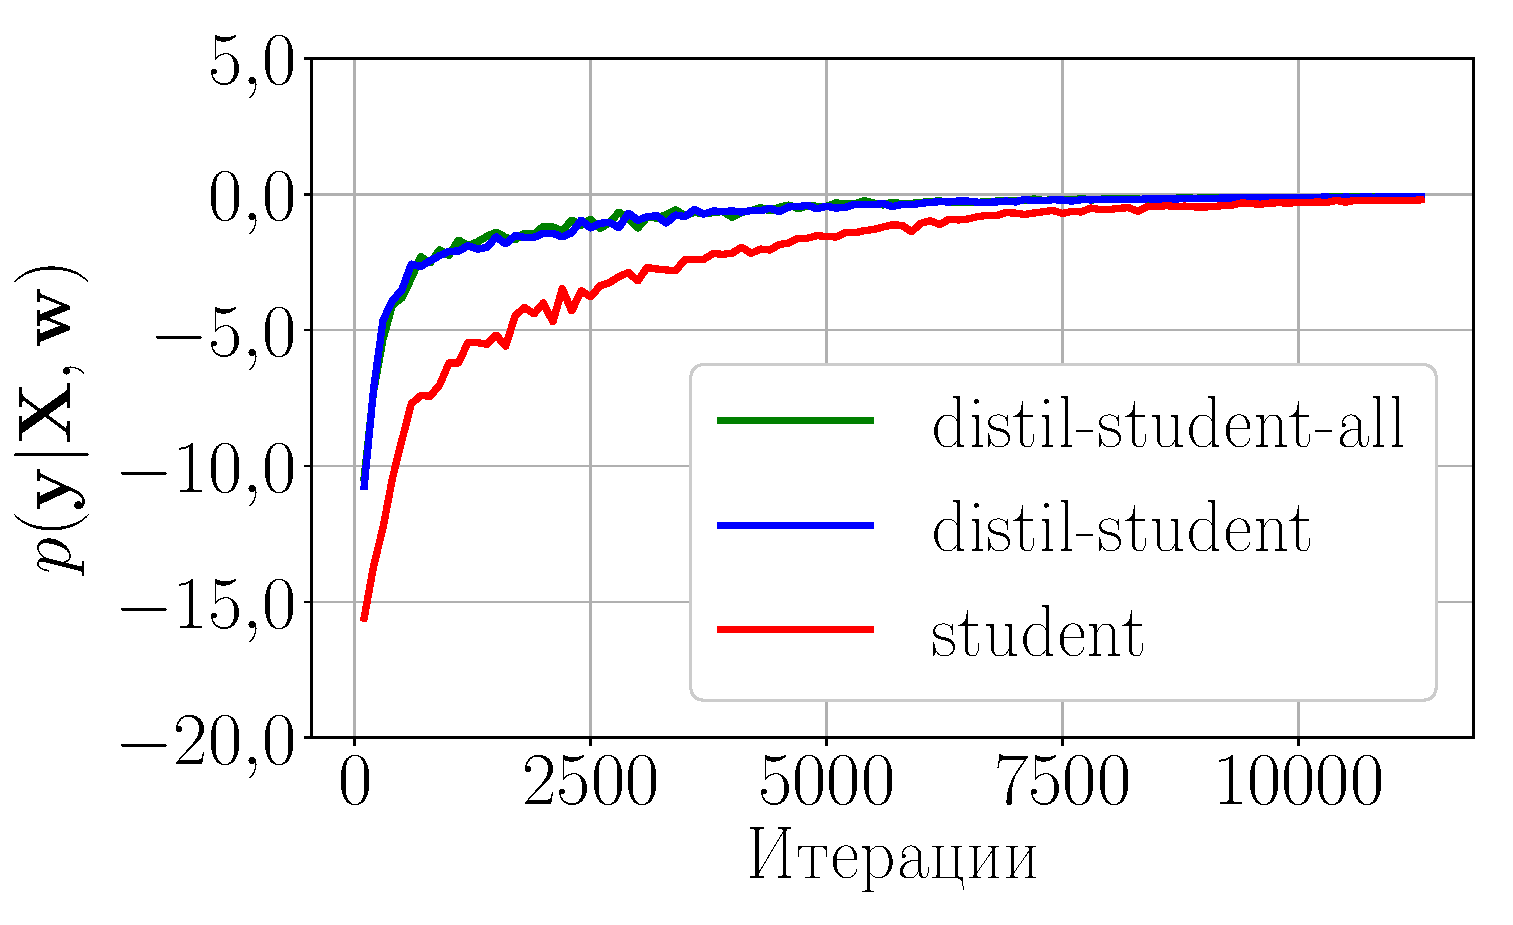
\includegraphics[width=0.5\textwidth]{results/bayesdistil/synthetic_likelihood_3_layers.eps}
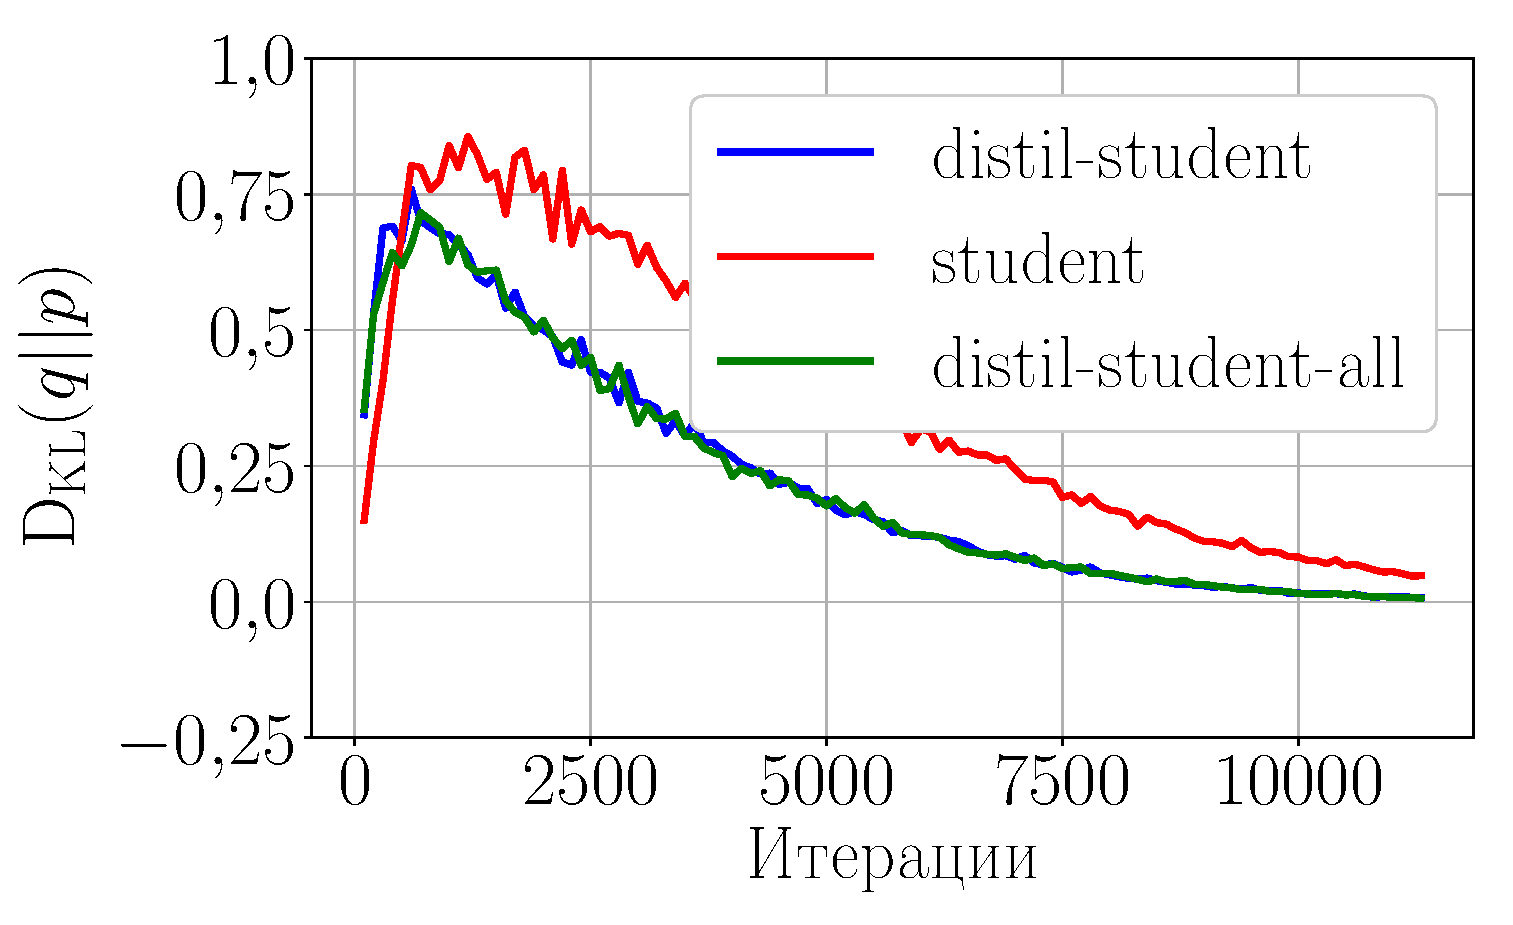
\includegraphics[width=0.5\textwidth]{results/bayesdistil/synthetic_D_KL_3_layers.eps}
\caption{Структура \eqref{ch:3:eq:ex:3} модели ученика $g$. Слева: правдоподобие выборки в зависимости от номера итерации при обучении. Справа: KL--дивергенция между вариационным и априорным распределениями параметров модели}
\label{ch:3:exp:fig1}
\end{figure}

Рис. \ref{ch:3:exp:fig1} сравнивает модели ученика, со структурой \eqref{ch:3:eq:ex:3}. Представлено сравнение разных моделей: модель без дистилляции, где в качестве априорного распределения выбирается стандартное нормальное распределение (на легенде обозначается student); модель с частичной дистилляцией, где в качестве среднего значения параметров выбираются параметры согласно выражения \eqref{ch:3:eq:ap:3}, а ковариационная матрица приравнивается к единичной матрицы (на легенде обозначается distil-student); модель с полной дистилляцией согласно выражения \eqref{ch:3:eq:ap:3} (на легенде обозначается distil-student-all). Видно, что обе модели ученика, где в качестве априорного распределения выбраны распределения, основанные на апостериорном распределении учителя, имеют большее правдоподобие, чем модель где в качестве априорного распределения выбрано стандартное нормальное~$\mathcal{N}\bigr(0,1\bigr)$. Также заметим, что использование параметра среднего из апостериорного распределения дает основной вклад при дистилляции, так как качество моделей distil-student и distil-student-all совпадает.

Вторая конфигурация получается путем удаления слоя модели учителя:
\[
\label{ch:3:eq:ex:5}
\begin{aligned}
g = \bm{\sigma} \circ \mathbf{W}_2\bm{\sigma} \circ \mathbf{W}_1,
\end{aligned}
\]
где $\bm{\sigma}$ является нелинейной функцией активации, а матрицы линейных преобразований имеют размер
\[
\label{ch:3:eq:ex:6}
\begin{aligned}
\mathbf{W}_{1} \in \mathbb{R}^{1 \times 50}, \quad \mathbf{W}_{2} \in \mathbb{R}^{50 \times 10}.
\end{aligned}
\]
В качестве функции активации выбрана~$\text{ReLu}$.

\begin{figure}[h!]
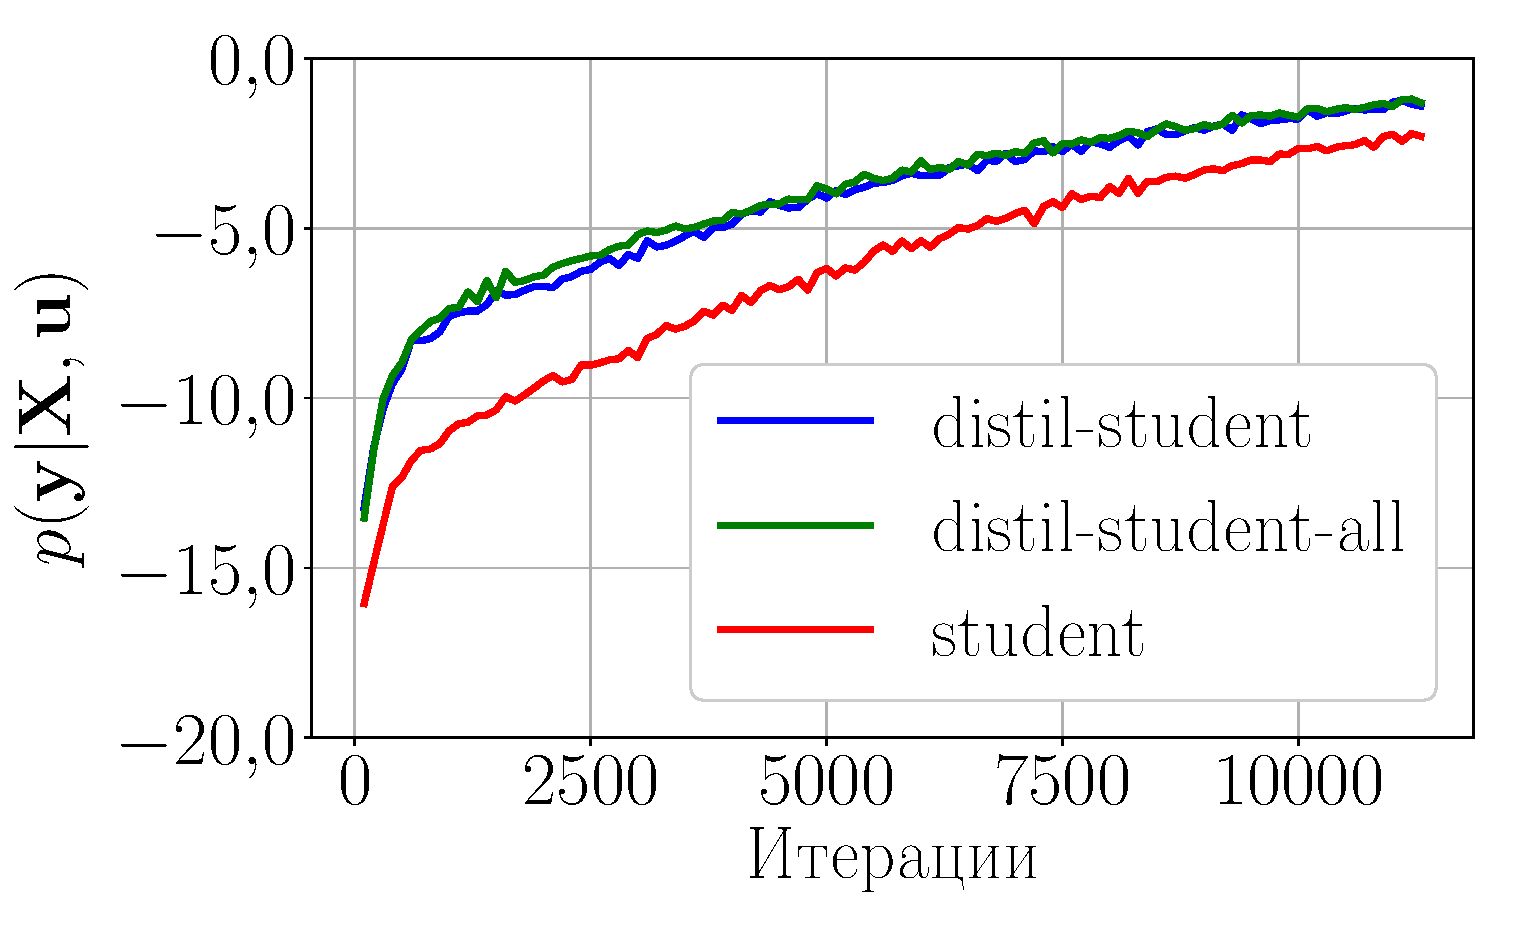
\includegraphics[width=0.5\textwidth]{results/bayesdistil/synthetic_likelihood_2_layers.eps}
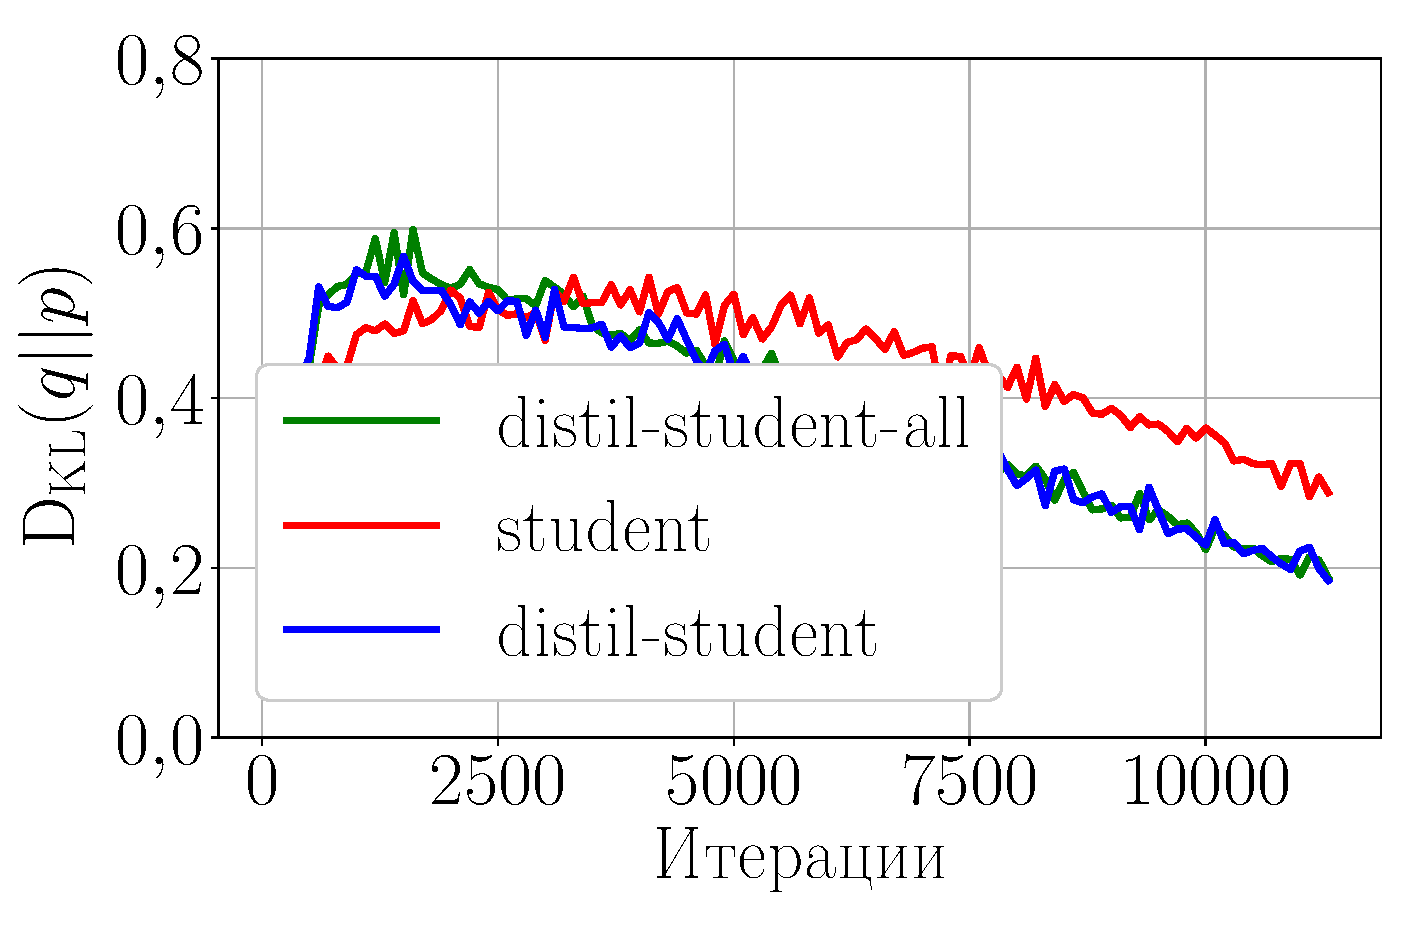
\includegraphics[width=0.5\textwidth]{results/bayesdistil/synthetic_D_KL_2_layers.eps}
\caption{Структура \eqref{ch:3:eq:ex:5} модели ученика $g$. Слева: правдоподобие выборки в зависимости от номера итерации при обучении. Справа: KL--дивергенция между вариационным и априорным распределениями параметров модели}
\label{ch:3:exp:fig2}
\end{figure}

Рис.~\ref{ch:3:exp:fig2} сравнивает модели ученика со структурой \eqref{ch:3:eq:ex:5}. Аналогично рис. \ref{ch:3:exp:fig1}, на рис. \ref{ch:3:exp:fig2} представлено сравнение модели без дистилляции (student), модели с дистилляцией параметра среднего значение (distil-student) и модели с полной дистилляцией (distil-student-all). В рамках данного эксперимента, по дистилляции модели учителя в модель ученика с меньшим числом параметров получены результаты, которые подтверждают, что задание априорного распределения параметров ученика позволяет снизить число итераций при выборе оптимальных параметров модели ученика.

В этой части эксперимента проводился анализ байесовского подхода к дистилляции на реальных данных.  В качестве реальных данных выбрана выборка FashionMnist~\cite{fashionmnist} описывающая задачу классификации изображений на 10 классов.

В качестве модели учителя рассматривался многослойный перцептрон с двумя скрытыми слоями \eqref{ch:3:eq:st:3}. Матрицы линейных преобразований имеют размер:
\[
\label{ch:3:eq:ex:7}
\begin{aligned}
\mathbf{U}_{1} \in \mathbb{R}^{800 \times 784}, \quad \mathbf{U}_{2} \in \mathbb{R}^{50 \times 800}, \quad \mathbf{U}_{3} \in \mathbb{R}^{10 \times 50},
\end{aligned}
\]
В качестве функции активации выбрана~$\text{ReLu}$.
Модель учителя предварительно обучена на основе вариационного вывода \eqref{ch:3:eq:st:7}, где в качестве априорного распределения параметров выбрано стандартное нормальное распределение.

В качестве модели ученика выбрана конфигурация с одним скрытым слоем \eqref{ch:3:eq:ex:5}, где матрицы линейных преобразований имеют размер:
\[
\label{ch:3:eq:ex:7}
\begin{aligned}
\mathbf{W}_{1} \in \mathbb{R}^{50 \times 784}, \quad \mathbf{W}_{2} \in \mathbb{R}^{50 \times 10}.
\end{aligned}
\]
В качестве функции активации выбрана~$\text{ReLu}$.

\begin{figure}[h!]
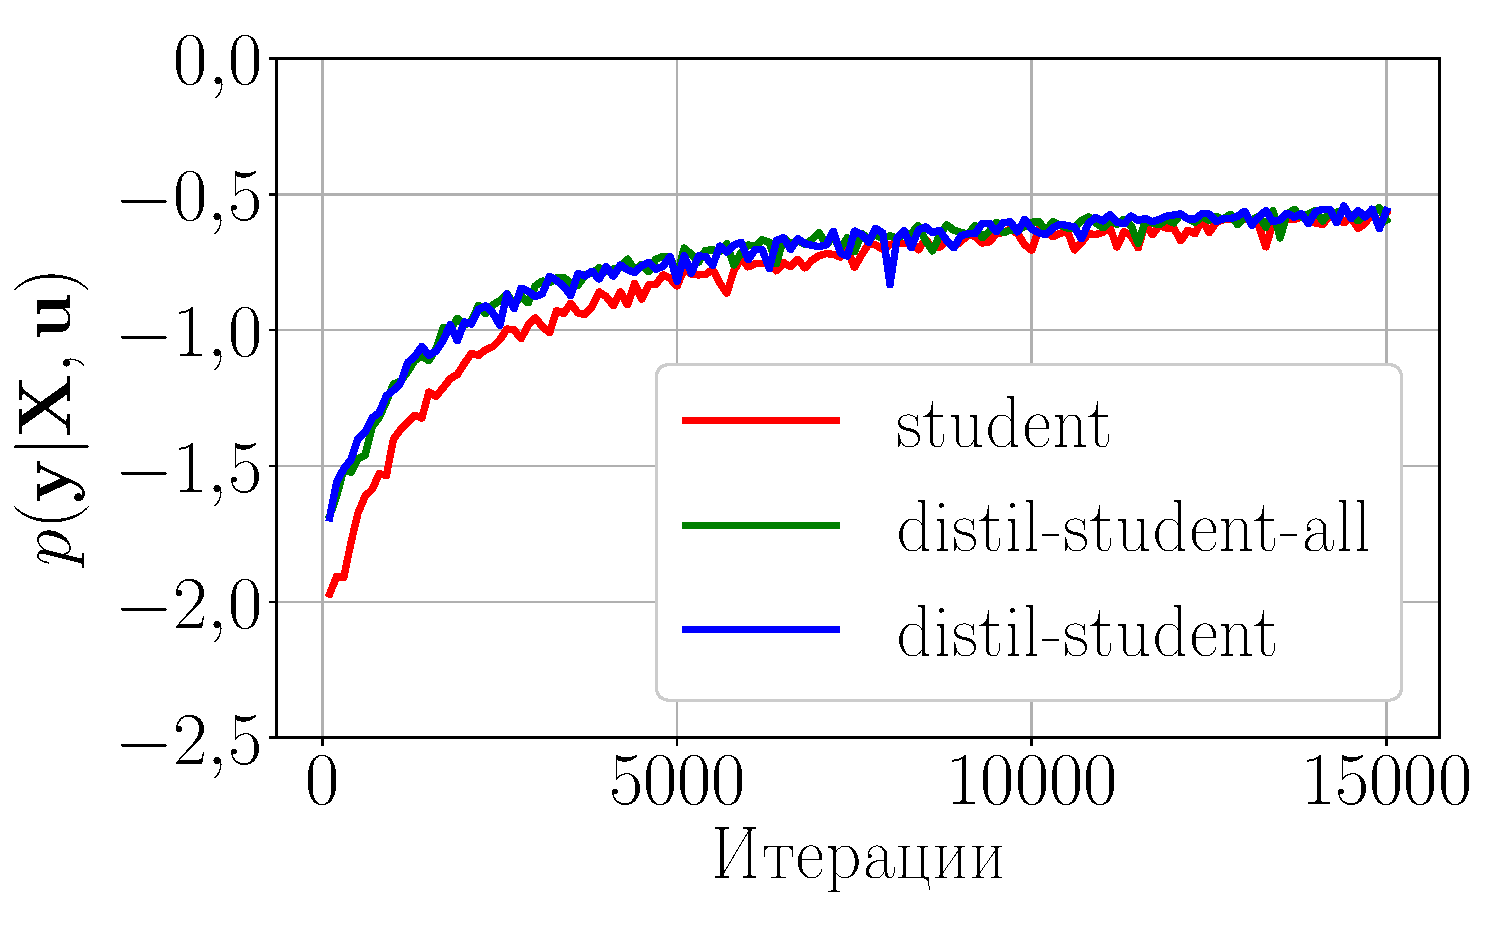
\includegraphics[width=0.5\textwidth]{results/bayesdistil/fashionmnist_likelihood_2_layers.eps}
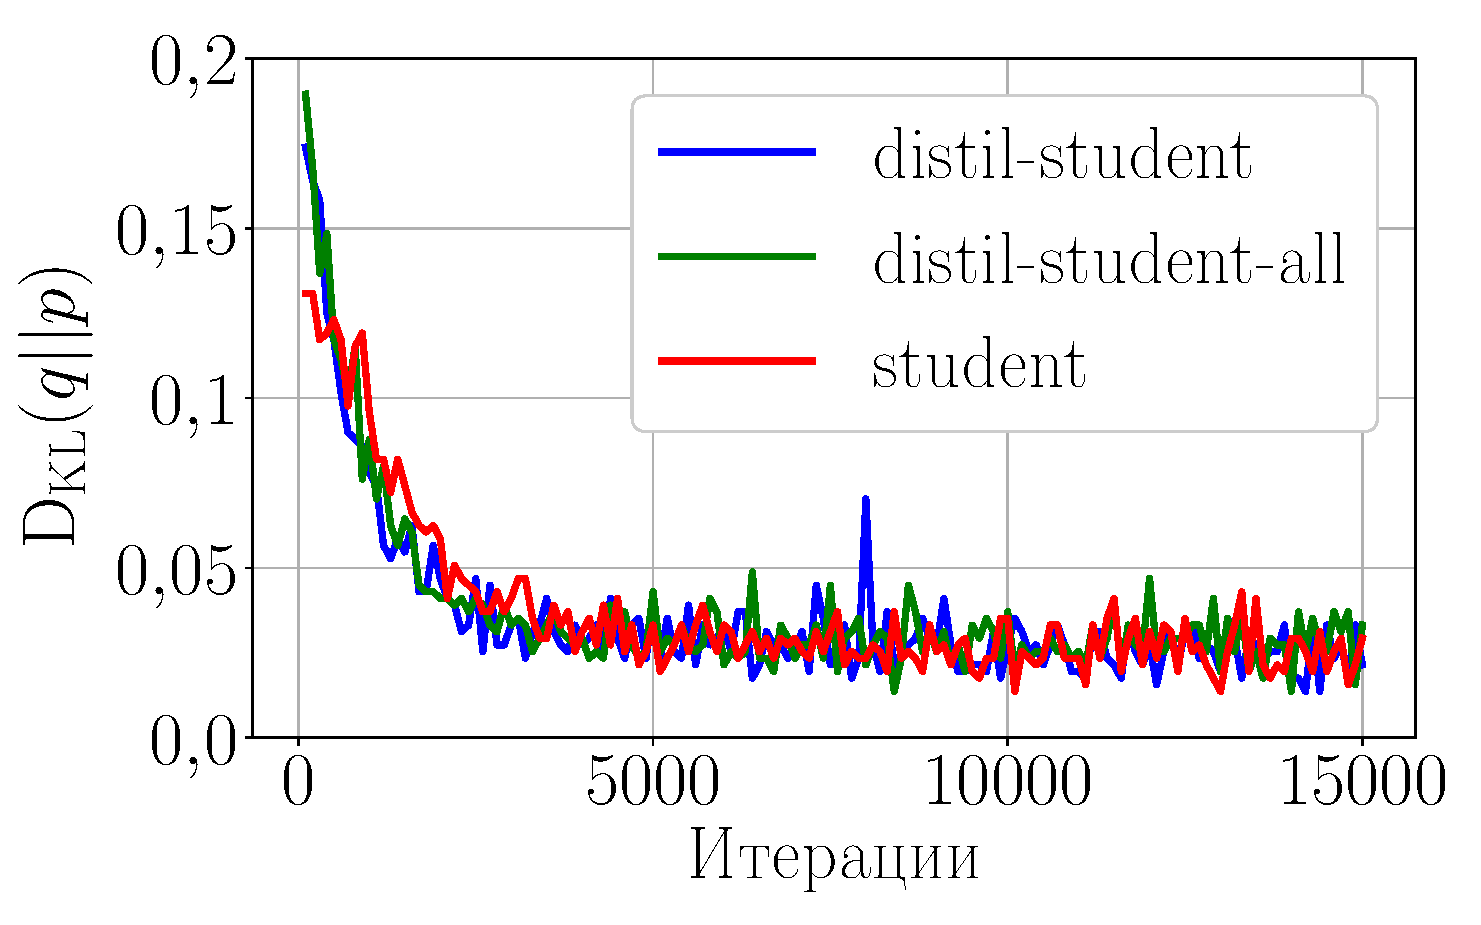
\includegraphics[width=0.5\textwidth]{results/bayesdistil/fashionmnist_D_KL_2_layers.eps}
\caption{Слева: правдоподобие выборки в зависимости от номера итерации при обучении. Справа: KL--дивергенция между вариационным и априорным распределениями параметров модели}
\label{ch:3:exp:fig3}
\end{figure}

Рис. \ref{ch:3:exp:fig3} сравнивает модели ученика с разными априорными распределениями параметров.
Аналогично синтетическому эксперименту, модель, где в качестве априорного распределения использовалось стандартное нормальное распределение, сравнивалась с моделью, где параметры распределения определялись на основе формулы \eqref{ch:3:eq:ap:5}. Видно, что у моделей с заданием априорного распределения на основе апостериорного распределения параметров учителя правдоподобие выборки выше, чем у модели, где в качестве априорного распределения выбрано стандартное нормальное распределение.

\begin{table}[]
\caption{Сводная таблица результатов анализа байесовской дистилляции}
\label{ch:3:tb:fn:1}
\begin{center}
\resizebox{\textwidth}{!}{
\begin{tabular}{|l|c|c|c|c|llll}
\cline{1-5}
                 & teacher           & student        & distil-student & distil-student-all &                           &                      &                      &                      \\ \cline{1-5}
\multicolumn{5}{|c|}{Эксперимент на синтетической выборке (удаление нейрона)}             &                      &                      &                      &                      \\ \cline{1-5}
Структура            & $[10,100,50,1]$   & $[10,10,10,1]$  & $[10,10,10,1]$ & $[10,10,10,1]$    &                      &                      &                      &                      \\ \cline{1-5}
Число параметров  & 6050                    & 210                   & 210                  & 210                      &                      &                      &                      &                      \\ \cline{1-5}
Разность площадей   &   -                         & 0                       & 16559              & 16864                  &                      &                      &                      &                      \\ \cline{1-5}
\multicolumn{5}{|c|}{Эксперимент на синтетической выборке (удаление слоя)}                    & \multicolumn{1}{c}{} & \multicolumn{1}{c}{} & \multicolumn{1}{c}{} & \multicolumn{1}{c}{} \\ \cline{1-5}
Структура            & $[10,100,50,1]$   & $[10,50,1]$       & $[10,50,1]$      & $[10,50,1]$          &                      &                      &                      &                      \\ \cline{1-5}
Число параметров    &   6050                       &          550                &          550               &             550                &                      &                      &                      &                      \\ \cline{1-5}
Разность площадей S    &  -                          &  0                      &  23310             & 25506                  &                      &                      &                      &                      \\ \cline{1-5}
\multicolumn{5}{|c|}{Эксперимент на выборке FashionMnist}                                                     &                      &                      &                      &                      \\ \cline{1-5}
Структура           & $[784,800,50,10]$& $[784,50,10]$   & $[784,50,10]$  & $[784,50,10]$      &                      &                      &                      &                      \\ \cline{1-5}
Число параметров    &           667700                  &          39700                &         39700                &                 39700            &                      &                      &                      &                      \\ \cline{1-5}
Разность площадей S   & -                           & 0                       &  1165               & 1145                    &                      &                      &                      &                      \\ \cline{1-5}
\end{tabular}
}
\end{center}
\end{table}

В табл. \ref{ch:3:tb:fn:1} представлен результат вычислительного эксперимента. Для численного сравнения качества моделей выбрана разность площадей графика правдоподобия $p\bigr(\mathbf{y}|\mathbf{X}, \mathbf{u}\bigr)$ между моделью student и моделями distil-student  и 
distil-student-all соответсвенно:
\[
\label{ch:3:eq:ex:8}
\begin{aligned}
S = \sum_{s} p\bigr(\mathbf{y}|\mathbf{X}, \mathbf{u}^s_{\text{s}}\bigr) - p\bigr(\mathbf{y}|\mathbf{X}, \mathbf{u}^s_{\text{ds}}\bigr),
\end{aligned}
\]
где $\mathbf{u}^s_{\text{s}}, \mathbf{u}^s_{\text{ds}}$ обозначает параметры модели студента и модели дистиллированного студента после $s$-й итерации оптимизационного процесса. Заметим, что площадь~$S$ имеет знак: чем больше значение положительного числа, тем дистиллированная модель точнее, чем модель построенная без учителя. Если площадь~$S$ принимает отрицательное значение, то это значит, что модель без дистилляции является точнее чем модель с дистилляцией. Из вычислительного эксперимента видно, что площадь~$S$ под графиками принимает положительные значения, то есть обе модели ученика полученные при помощи дистилляции, являются точнее чем модель ученика без дистилляции.